\documentclass[a4paper,12pt]{article}
\usepackage{amsmath}
\usepackage{amscd}
\usepackage{mathtext}
\usepackage{amsfonts}
\usepackage[english,russian]{babel}
\usepackage[utf8]{inputenc}
\usepackage[T2A]{fontenc}            % внутренняя кодировка  TeX
\usepackage{graphicx}
\usepackage{textcomp}
\usepackage{geometry}
\geometry{left=3cm}
\geometry{right=1.5cm}
\geometry{top=2cm}
\geometry{bottom=2cm}
\usepackage{tikz}
\usepackage{tikz-cd}
\usepackage{titling}
\usepackage{indentfirst}
\setlength{\parindent}{1cm}
\usepackage{soul}
\usepackage{enumitem}
\makeatletter
\AddEnumerateCounter{\asbuk}{\russian@alph}{щ}
\makeatother

\pretitle{\begin{flushleft}\Large\textbf}
\title{Декомпозиция линейных автоматов над кольцом вычетов в сдвиговые регистры \protect\footnote{Результаты приведённые в данной работе являются частью докторской диссертации автора, которой руководил профессор Урс Вюрглер (Urs Würgler) из Бернского университета.}}
\posttitle{\end{flushleft}}

\preauthor{\begin{flushleft}}
\author{Арнольд Шойинг (Arnold Scheuing)}
\postauthor{\end{flushleft}}

\predate{\begin{flushleft}}
\date{\textit{\scriptsize{Институт информатики и прикладной математики, Бернский университет, CH-3012 Берн, Швейцария}}}
\postdate{\end{flushleft}}

\newcommand{\dirsummod}[1]{{_{{#1}}\!\!\sum}}

\newcommand{\hatei}[1]{\hat{e}_{#1}}

\newcommand{\Ann}{\text{Ann}}

\newcommand{\im}{\text{im}}

\newcommand{\Endom}{\text{End}}

\newcommand{\coker}{\text{coker}}



\newcommand{\Hom}{\text{Hom}}
\newcommand{\Aut}{\text{Aut}}
\newcommand{\Rad}{\text{Rad}}
\newcommand{\Mod}{\text{Mod}}

\begin{document}


\maketitle

\begin{abstract}
	Линейный автомат $\mathfrak{A}$ над факторкольцом $\mathbb{Z}_{n}$, $n \in \mathbb{N}$, в общем случае неразложим на параллельно соединённые сдвиговые регистры. Мы смогли сформулировать необходимые и достаточные условия для такого разложения, используя торию об артиновых локальных кольцах $R$ и $R[x]$-модульной структуре $\mathfrak{A}$.

\end{abstract}

\section{Введение}

Структура конечного, детерминированного линейного автомата (далее КА) интересна не только с точки зрения информатики, но и с точки зрения теории систем. Сфера применений КА, называемых также линейными последовательными схемами (LCS) включает в себя обнаружение и исправление ошибок, генераторы случайных чисел, криптологию (мотивация автора), а также конечномерные линейные системы с постоянными коэффициентами и дискретным или непрерывным временем. До тех пор пока коэффициенты такого автомата или системы являются элементами поля $F$, структура хорошо известна и тщательно изучалась последние двадцать лет \cite{bib4} с помощью линейной алгебры: пространство состояний $E$ автомата $\mathfrak{A}$ --- это конечномерное векторное пространство $E$ над $F$, а функция перехода может быть рассмотрена как эндоморфизм в $E$ или как матрица $A$ над $F$, если базис в $E$ зафиксирован.

Для нахождения более "простого" эквивалентного $\mathfrak{A}$ КА можно использовать взаимооднозначное соответствие между КА, эквивалентными $\mathfrak{A}$, и матрицами, подобными $A$. Есть существенные причины для выбора рациональной канонической формы $A$ как наиболее "простой", потому что она соответствует разложению $A$ на параллельные сдвиговые регистры.

На рисунке \ref{fig1abc} мы показываем три представления КА относительно данного базиса $B$ в $E$. Рисунок \ref{fig1abc}(а) соответствует сдвиговому регистру (его технической реализации) с 3-мерным пространством состояний, каждое из которых обладает компонентами $(s_1, s_2, s_3)$. В теории систем $s_i$ и $a_i$ называются, соответственно, элементами задержки и умножения. Каждый такт элемент из $s_3$ переходит в $s_2$, из $s_2$ --- в $s_1$ и сумма $a_0 s_1 + a_1 s_2 + a_2 s_3$ (в поле $F$) попадает в $s_3$. На рисунке \ref{fig1abc}(б) изображено представление линейной функции $f$ в форме матрицы $3 \times 3$. Эта специальная форма называется сопровождающей матрицей. Если полином $x^3 - a_2 x^2 - a_1 x - a_0$ является несократимым в $F[x]$, тогда КА нельзя разложить. Рисунок \ref{fig1abc}(в) указывает $F[x]$-модуль ранга 3, например, базис $B$ имеет три элемента: $e$, $f(e)$, $f^2(e)$, и
$$
f^3(e) = a_0 e + a_1 f(e) + a_2 f^2(e).
$$

\begin{figure}[h]
	\centering
	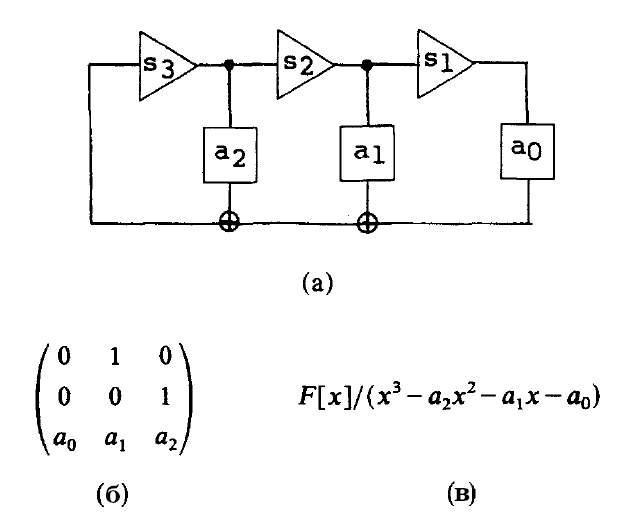
\includegraphics[width=0.5\linewidth]{pictures/fig1abc.png}
	\caption{Соответствующие представления $(a_0, a_1 , a_2 \in F)$. (а) Сдвиговый регистр. (б) Сопровождающая матрица. (в) Циклический F[x]-модуль ранга 3.}
	\label{fig1abc}
\end{figure}

Взаимооднозначное соответствие между этими структурами используется на всём протяжении данной работы: диаграммы КА и сдвиговые регистры для визуализации технической реализации, матрицы для расчётов в примерах, а модули для развития теории.

Известно, что КА с коэффициентами над полем может быть всегда реализован с помощью параллельного соединения сдвиговых регистров \cite{bib9}. Но в применениях, указанных выше, нас также интересуют системы над кольцами $\mathbb{Z} \mod 2^r (r \in \mathbb{N})$. Например, в криптологии процесс автоматизированного шифрования и расшифрования связан с диапазоном значений $2^r$ регистра с $r$ бинарными разрядами.

Хорошее исследование расширения теории линейных систем от полей до колец за последние десять лет можно найти в работе \cite{bib12}. Принцип двойственности для линейных систем над факторкольцами рассматривалась в работах \cite{bib2,bib8}. Представление матричных дробей для линейных систем над коммутативными кольцами также было изучено в работе \cite{bib5}.

В разделе 5 мы приводим пример КА над $\mathbb{Z}_4$, который и не является, и не разложим на сдвиговые регистры. Следовательно, возникает вопрос, при каких условиях КА над $\mathbb{Z}_n$ может быть реализован как параллельное соединение сдвиговых регистров. Похожая проблема изучалась в работах \cite{bib6, bib7}, путём использования биекции $\beta : \mathbb{Z}_{p^r} \approx \prod_{1}^{r}\mathbb{Z}_p$ для декомпозиции КА $\mathfrak{A}$ над $\mathbb{Z}_{p^r}$ в каскад из $r$ автоматов $\mathfrak{A}_i$ над $\mathbb{Z}_p$. Но поскольку $\beta$ не является гомоморфизмом колец, $\mathfrak{A}_i$ соединены с помощью нелинейной логикой без задержек, которая ограничивает дальнейший анализ посредством коммутативной алгебры.

Данная работа состоит из следующих разделов: в разделе 2 мы покажем, что $\mathbb{Z}_{n}$-свободные $\mathbb{Z}_{n}[x]$-модули являются подходящими математическими объектами для изучения структуры КА над полем $\mathbb{Z}_{n}$ (рисунок \ref{fig1abc}). В разделе 3 мы докажем что проблема может быть сведена к КА над $\mathbb{Z}_{p}$ без потери общности; с другой стороны, рекурсивный критерий в последнем разделе предлагает не ограничивать наше внимание на конечных и локальных кольцах $\mathbb{Z}_{p^r}$, а рассматривать более общие (коммутативные) артиновы локальные кольца $R$ (с 1). Следовательно, в разделе 3 мы соберём все необходимые утверждения относительно артиновых локальных колец и модулей над ними. В разделе 4 мы покажем, что наш $R[x]$-модуль всегда имеет примарное разложение. Основные результаты находятся в разделах 5 и 6, где мы приводим необходимые и достаточные условия для циклического разложения пространства состояний; другими словами, условия для того, чтобы КА был эквивалентен прямой сумме сдвиговых регистров. Общий случай мы рассматриваем в разделе 5, а специальный с кольцом главных идеалов --- в разделе 6.


\section{Модульная структура конечного автомата}

Начнём с более точного описания конечного автомата (КА).

\paragraph{Определение 2.1}

Конечный детерминированный линейный автомат (без входных или выходных функций) над кольцом $R$ --- это пара $(E,f)$, где пространство состояний $E$ является свободным $R$-модулем конечной размерности (скажем $n$), а функция перехода $f$ --- это линейное отображение из $E$ в $E$. Каждое $e \in E$ является состоянием КА, функция перехода отображает состояние $e$ в новое $f(e)$. Мы можем использовать простую нотацию без начального состояния, потому что нас интересует структура КА в целом.

Множество функций переходов над $E$ --- это кольцо эндоморфизмов $\Endom_R(E) = \{f : E \rightarrow E ~| ~f~ линейна\}$. $\Endom_R(E)$ также является $R$-модулем. Этот факт может быть выражен с помощью гомоморфизма колец на следующей коммутативной диаграмме.

\begin{figure}[h]
	\centering
	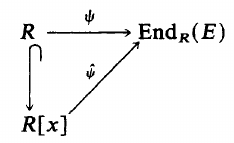
\includegraphics[width=0.25\linewidth]{pictures/diag_1.png}
%	\label{diag_1}
\end{figure}

Для $r \in R$, $\psi(r)$ --- это скалярное произведение для $r$ из $E$. Так как $f$ линейна над $E$, мы можем расширить $\psi$ на $R[x]$ как гомоморфизм колец с помощью задания $\hat{\psi}(x) := f$. Теперь $E$ становится $R[x]$-модулем.

Путём параллельного соединения различных КА над одним и тем же кольцом мы можем построить более крупный автомат. Но ещё больший интерес представляет возможность разложения данного (сложного) автомата на мельчайшие, несократимые части --- сдвиговые регистры.

\paragraph{Определение 2.2}
КА $(E,f)$ над кольцом $R$ называется \textit{сдвиговым регистром}, если $E$ цикличное, как $R[x]$-модуль. Другими словами, если существует такое начальное состояние $e \in E$, что его орбита:
$$
e, f(e), f^2(e), ..., f^{n-1}(e)
$$
охватывает $E$.

Под "<параллельным соединением КА $(E_i, f_i)$"> мы подразумеваем техническую реализацию (см. рисунок \ref{fig2ab}(б)), но оно попросту означает прямую сумму КА $(\bigoplus{E_i}, \bigoplus{f_i})$. Высказывание "<КА реализован как параллельное соединение сдвиговых регистров"> является интуитивным способом выразить то, что $E$ --- это прямая сумма $R[x]$-цикличных $R$-свободных подмодулей.

Для формулировки первой теоремы необходима следующая нотация:

\begin{itemize}
	\item $M_n(R)$ --- множество всех $n \times n$-матриц над $R$,
	\item $GL_n(R)$ --- подмножество всех регулярных матриц из $M_n(R)$,
	\item $M_n(R)/GL_n(R)$ --- множество всех классов подобия матриц ($A \in M_n(R)$ подобна $T^{-1}AT$ для всех $T \in GL_n(R)$),
	\item $\Mod_n(Rp[x])$ --- класс всех $R$-свободных $R[x]$-модулей $E$ ранга $n$ (т.е. $dim_R(E) = n$),
	\item $Iso(\Mod_n(R[x]))$ --- множество классов изоморфизма таких модулей.
\end{itemize}


\paragraph{Теорема 2.3}{\itshape
Существует биекция:
$$
\chi : M_n(R)/GL_n(R) \rightarrow Iso(\Mod_n(R[x]))
$$
}

\paragraph{Доказательство.}
\hl{Определение $\chi$: Пусть $[A] \in M_n(R)/GL_n(R) ~ и ~ A \in M_n(R)$ --- представители (Definition of $\chi$: Let ... be a representant.)}.
Далее, пусть $E$ --- свободный $R$-модуль ранга $n$. Выберем базис в $E$ и определим $x \cdot e := A \cdot e ~ (\forall e \in E)$. Таким образом $E$ становится $R[x]$-модулем $E_A$. Определим $\chi [A] := [E_A]$ --- класс изоморфизма $E_A$. $\chi$ определено корректно, потому что для подобных матриц $A \sim A'$, модули изоморфны: $E_A \cong E_{A'}$, следовательно, $[E_A] = [E_{A'}]$.

Определение $\chi'$: \hl{Пусть $[F] \in Iso(\Mod_n(R[x])) ~ и ~ F \in \Mod_n(R[x])$ --- представители (Definition of $\chi$: Let ... be a representant.)}. Выберем $R$-базис в $F$, тогда (линейное) преобразование $x$ может быть выражено с помощью матрицы $A$. Если мы зададим $\chi'[F] := [A]$, то оно также корректно определено и очевидно является обратной функцией к $\chi$.  $\Box$

\section{Артиновы локальные кольца и конечнопорождённые модули}

В первой части этого раздела мы применим китайскую теорему об остатках для упрощения задачи с КА над $\mathbb{Z}_{n}$ до КА над $\mathbb{Z}_{p^r}$ ($p$ --- простое, $r \in \mathbb{N}$).
Мы помним, что кольцо $\mathbb{Z}_{n}$ изоморфно произведению колец $\prod_{i=1}^{m} { {\mathbb{Z}}_{{p_{i}^{r_{i}}}}}$, так как $n$ единственным образом разлагается на простые множители $n = p_1^{t_1} p_2^{t_2} \cdot \cdot \cdot p_m^{t_m}$. Из этого изоморфизма вытекает следующая теорема. 

\paragraph{Теорема 3.1}{\itshape
Пусть $R_1, R_2, ..., R_m$ --- (коммутативные) кольца (с единицей), $R:=\prod_{i=1}^{m}R_i$, $E$ --- $R$-модуль и определим $E_i := E \otimes R_i$. Тогда кольцо $\Endom_R(E)$ изоморфно $\bigoplus_{i=1}^{m}\Endom_{R_i}(E_i)$.
}
\paragraph{Доказательство.}
Пусть $f_i := f\otimes1_{E_i} \in \Endom_{R_i}(E_i)$. Мы можем определить гомоморфизм колец $\phi : \Endom_R(E) \rightarrow \bigoplus_{i=1}^{m} \Endom_{R_i} (E_i)$ как $\phi(f) := (f_1, f_2, ..., f_m)$. 

Если $\phi$ --- мономорфизм: для $f \in ker(\phi) \Rightarrow f_i = f \otimes 1_{E_i} = 0 (\forall i) \Rightarrow f(E) \cong \prod_{i}(f(E) \otimes R_i) = 0 \Rightarrow f = $ \hl{(ОПЕЧАТКА: в оригинальной статье формула обрывается).}

Если $\phi$ --- эпиморфизм: мы выбираем произвольное $f_i \in \Endom_{R_i} (E_i)$. Принимая во внимание диаграмму:

\begin{figure}[h]
	\centering
	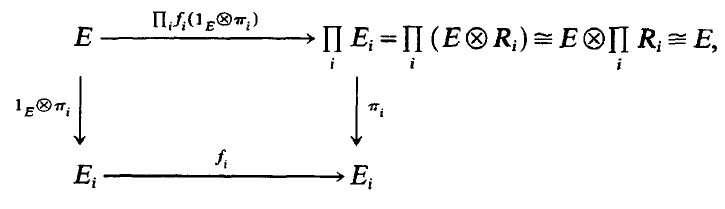
\includegraphics[width=0.5\linewidth]{pictures/diag_2.png}
	%\label{diag_2}
\end{figure}

получаем, что $\phi(\prod_i f_i (1_E \otimes \pi_i)) = (f_1, f_2, ..., f_m)$. $\Box$

\paragraph{Следствие 3.2}
КА над $\mathbb{Z}_n$ может быть всегда реализован с помощью параллельного соединения КА над $\mathbb{Z}_{p^r}$.


\paragraph{Пример 3.3}
КА над $\mathbb{Z}_6$, изображенный на рисунке \ref{fig2ab}(a), изоморфен автомату на рисунке \ref{fig2ab}(b). Соответствующий модуль выглядит следующим образом:
$$
E \cong \mathbb{Z}_6 [x] / (x^3 - 2x^2 - 3x - 4) \cong \mathbb{Z}_2 [x] / (x^3 + x) \oplus \mathbb{Z}_3 [x] / (x^3 + x^2 - 1).
$$

Во второй части данного раздела мы хотим собрать воедино необходимые факты об артиновых локальных кольцах и о модулях над ними.

\begin{figure}[h]
	\centering
	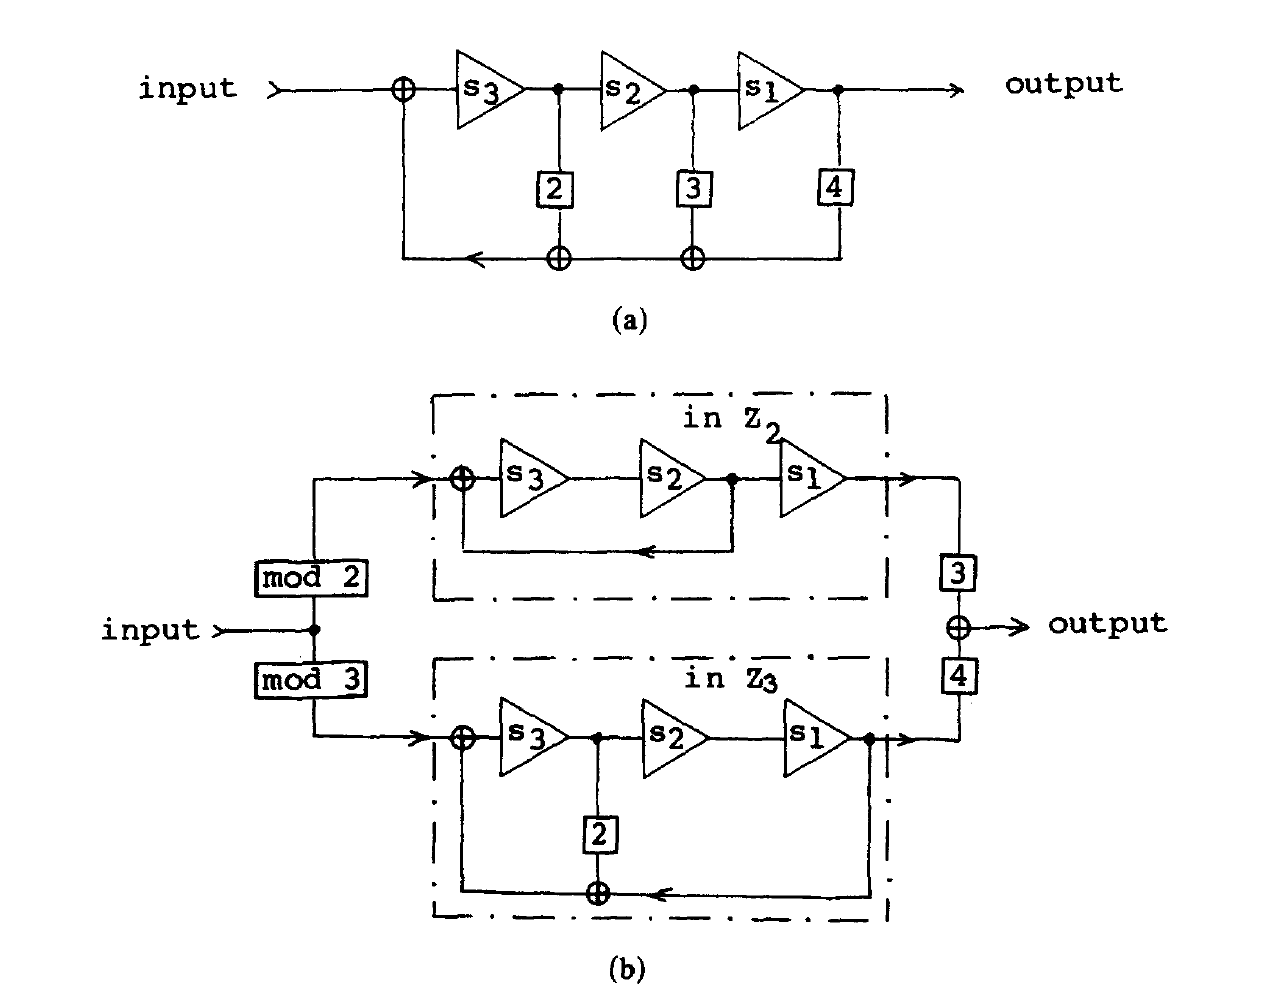
\includegraphics[width=0.75\linewidth]{pictures/fig2ab.png}
	\caption{Эквивалентные КА над $\mathbb{Z}_6$ (со входом и выходом)}
	\label{fig2ab}
\end{figure}

\paragraph{Определение 3.4}
Кольцо $R$ является артиновым, если оно нётерово и имеет размерность 0 (любой простой идеал максимален, см. \cite{bib1}).

Кольцо $R$ является локальным, если оно нётерово и имеет ровно один максимальный идеал $M$. Нотация: $(R,M)$.

\paragraph{Пример 3.5}
$(\mathbb{Z}_{p^r}, (p))$ и $(\mathbb{Z}_{p^r}[x]/(x^S), (p,x))$ --- это артиновы локальные кольца.

\paragraph{Лемма 3.6}{\itshape
Артиновы локальные кольца $(R,M)$, обладают следующими свойствами:
}

\renewcommand{\labelenumi}{(\asbuk{enumi})}
\begin{enumerate}
	\item М является единственным простым идеалом;
	\item нильрадикал $\Rad(R)$ совпадает с $M$ и сам является нильпотентным; наименьшее $z \in \mathbb{N}$, при котором $M^z = (0)$, называется нильпотентностью $M$;
	\item каждый элемент $R$ либо обратим, либо нильпотентен.
\end{enumerate}

Снэппер (Snapper) \cite{bib11} называет такие кольца "<совершенно простыми кольцами">.

Учитывая важность канонического отображения $\pi : R \rightarrow R / \Rad(R)$, мы будем использовать следующую нотацию на всём протяжении работы: $\overline{R} = R / \Rad(R)$, поле вычетов, $\overline{r} = \pi (r) (\forall r \in R), \overline{M[x]} = \pi (M[x]) = 0$.

\paragraph{Примечание 3.7}
В данной работе мы будем рассматривать только конечнопорождённые модули, не повторяя этот факт каждый раз.\\

Причина, по которой мы не можем следовать такому же разложению, как для автомата над полем $F$ (т.е. как модули над областью главных идеалов $F[x]$), состоит в том, что подмодуль свободного модуля не обязательно является свободным. Но у нас есть следующая фундаментальная теорема.

\paragraph{Теорема 3.8}
{\itshape
(а) В локальном кольце $(S, M)$ все конечнопорождённые модули свободны.

(б) Пусть $(S, M)$ --- артиново локальное кольцо, $F \subset E$ --- оба конечнопорождённые свободные $S$-модули. Тогда $E \cong F \oplus E/F$.

(в) Пусть $(S, M)$ артиново локальное кольцо, $F, G \subset E$ --- три конечнопорождённых свободных $S$-модуля. Тогда $F \cap G$ и $F + G$ являются свободными. 
}

\paragraph{Доказательство.}
(а) См. \cite{bib10}.

(б) Пусть $\{e_1, ..., e_n\}$ и $\{f_1, ..., f_m\}$ --- базисы в $E$ и $F$, соответственно. Поскольку $F \cap E \Rightarrow f_1 = \sum \phi_i e_i$ и поскольку $\{f_1, ..., f_m\}$ линейно независимы, как минимум один из $\phi_i$ должен быть обратим (см. лемму 3.6). Без потери общности, обратимый $\phi_i$ подразумевает $e_1 = (\phi_1^{-1})(f_1 - \sum_{i < 1} \phi_i e_i)$. Поэтому $\{f_1, e_2, ..., e_n\}$ --- это базис в $E$. По индукции получаем, что $\{f_1, f_2, ..., f_m, e_{m+1}, ..., e_n\}$ является базисом в $E$, следовательно, $E \cong F \oplus L_R (e_{m+1}, ..., e_n)$.

(в) $G \rightarrow F \oplus E/F$ и оба слагаемых свободные (см. часть (б)). Пусть $\{g_1,...,g_p\}$ --- базис в $G$, а $\{f_1, f_2, ..., f_m, e_{m+1}, ..., e_n\}$ --- базис в $E =  F \oplus E/F$. Поскольку $g_i \in E$, мы можем заключить аналогично части (б), что $\{g_1, ..., g_q, f_{q+1}, ..., f_m, g_{q+1}, ..., g_p, e_{n-m-p+q}, ..., e_n\}$ является базисом в $E$. Следовательно, $F \cap G = L_S(g_1, ..., g_q)$ и $F + G = L_S(g_1, ..., g_p, f_{q+1}, ..., f_m)$ свободны. $\Box$ \\

Напомним, что для несократимого полинома $\alpha \in R[x]$, \hl{отображение (projection)} $\overline{\alpha} \in \overline{R}[x]$ не обязательно будет несократимым. Если оно является таковым, то мы называем $\alpha$ фундаментально несократимым.


\paragraph{Лемма 3.9}{\itshape
Вот некоторые важные типы идеалов в $R[x]$ для артинова локального $(R, M)$:

\renewcommand{\labelenumi}{(\asbuk{enumi})}
\begin{enumerate}
	\item $M[x] := \{\sum_i r_i x^i \in R[x] | r_i \in M \} \subset R[x]$ является единственным \hl{нулевым (nil)} простым идеалом в $R[x]$;
	\item Все ненулевые простые идеалы имеют вид $M[x] + (\alpha)$, где $\alpha \in R[x]$ приведённый и фундаментально несократимый. Поскольку $\overline{R}$ поле, эти идеалы также являются максимальными;
	\item Ненулевой идеал в $R[x]$ представим в виде $N + (\beta)$, где $\beta$ --- приведённый многочлен и $N \subset M[x]$. Порождающие $N$ могут быть всегда выбраны так, что их степень будет меньше, чем $\beta$.
\end{enumerate}
}

Доказательство очевидно; подробности можно найти в работе \cite{bib11}.

\section{Примарное разложение}
Для начала подготовим факты и определения, связанные с идеалами. Пусть $J$ --- идеал в кольце $S$.
Радикал в $J$ --- это $\Rad(J) = \{s \in S | \exists n \in \mathbb{N}: s^n \in J\}$. Напомним, что $\Rad(R) := \Rad(0)$. $J$ называется примарным, если для $s t \in J, t \notin J \Rightarrow s \in \Rad(J)$.

Пусть $E$ --- это $S$-модуль, тогда аннигиляторный идеал в $E$ определяется как $\Ann_S(E) := \{s \in S | s e = 0 (\forall e \in E)\}$.

\paragraph{Определение 4.1}
$S$-модуль называется примарным, если $(0)$ --- это примарный подмодуль $E$. То есть $s e = 0$ (при $s \in S$, $0 \ne e \in E$) означает, что $s \in \Rad(\Ann_S(E))$. (Если элемент $s$ уничтожает один элемент из $E$, то мощность $s$ уничтожает всё в $E$.) Идеалы $J$ и $I$ в $S$ называются взаимно простыми, если $I + J = S$.

\paragraph{Лемма 4.2}
{\itshape
Пусть $(R, M)$ --- артиново локальное кольцо и $I$, $J$ --- примарные идеалы в $R[x]$. Тогда:
\renewcommand{\labelenumi}{(\asbuk{enumi})}
\begin{enumerate}
	\item $J, I$ взаимно простые $\Leftrightarrow ~ \Rad(J)$, $\Rad(I)$ взаимно простые;
	\item Пусть $J$ и $I$ ненулевые: $\Rad(J) = \Rad(I) \Rightarrow J$ и $I$ взаимно простые.
\end{enumerate}
}

\paragraph{Доказательство}
(а) ($\Leftarrow$): Очевидно, так как $\Rad(J) \subset J$ и $\Rad(I) \subset I$.

$(\Rightarrow)$: Выберем $p \in \Rad(J), q \in \Rad(I)$ такими, что $p + q = 1$. Теперь существуют такие $n, m \in \mathbb{N}$, для которых выполняется $p^m \in J$ и $q^n \in I$, что:
$$
1 = 1^{m+n-1} = (p + q)^{m+n-1} = \sum_{k=1}^{m+n-1} \binom{m+n-1}{k}p^k \cdot q^{m+n-k-1} = p^m (...) + q^n (...) ~ \in J+I,
$$
что подразумевает $1 \in I+J$.

(б) Из леммы 3.9 мы знаем что $\Rad(J) = M[x] + (\alpha), \Rad(I) = M[x]+(\beta)$, где подходящие $\alpha, \beta \in R[x]$ нормированы, а $\overline{\alpha}, \overline{\beta)} \in \overline{R}[x]$ взаимно просты. Следовательно, $1 \in (\overline{\alpha}) + (\overline{\beta})$, и $1 + \nu \in (\alpha) + (\beta)$ для некоторого $\nu \in M[x]$. Таким образом, $\Rad(J)$ и $\Rad(I)$ взаимно простые и, учитывая часть (а), $J$ и $I$ взаимно простые.
$\Box$

\paragraph{Лемма 4.3}
{\itshape
Пусть $R$ --- нётерово кольцо, и $E$ --- $R$-свободный R[x]-модуль. $E$ является примарным тогда и только тогда, когда $\Ann_{R[x]}(E)$ является примарным.
}

\paragraph{Доказательство}
Пусть $A := \Ann_{R[x]}(E)$.

($\Rightarrow$): Допустим $\alpha \beta \in A, \beta \notin A$, подразумевая, что существует $0 \ne e \in E$, для которого $\beta e \ne 0$. Но $(\alpha \beta)e = 0 = \alpha (\beta e)$ и $E$ примарный, следовательно, $\alpha \in \Rad(A)$.

($\Leftarrow$) Пусть $0 \ne e \in E, \alpha e = 0$. Мы знаем, что
$$((\alpha)+A) \cdot ((\alpha) \cap A) ~~ \subset ~~ (\alpha) \cdot A ~~ \subset ~~ (\alpha) \cap A.$$

\textit{Случай} 1: $(\alpha) \cdot A = (\alpha) \cap A$. Для нётеровых колец это означает, что $(\alpha) + A = R[x]$. Следовательно, существуют такие $\beta \in R[x]$ и $\gamma \in A$, что $\beta \alpha + \gamma = 1$. Возникает противоречие: $1 \cdot e = \beta (\alpha e) + \gamma e = \beta 0 + 0$. 

\textit{Случай} 2: $(\alpha) \cdot A \ne (\alpha) \cap A$. Существует $\beta \in (\alpha) \cap A, \beta \notin (\alpha) \cdot A$ такое, что $\beta = \alpha \gamma \in A, \gamma \notin A$, следовательно, $\alpha \in \Rad(A)$. $\Box$ \\

Нас интересуют артиновы локальные кольца, а они по определению являются нётеровыми, поэтому мы можем применить следующую важную теорему.

\paragraph{Теорема 4.4}
{\itshape
В нётеровом кольце $R$ каждый идеал имеет примарное разложение на примарные идеалы $Q_i$ (с точностью до порядка \hl{(unique up to order)})
$$
J = \bigcap_{i=1}^{m} Q_i, ~~~~~ Q_i \not \subset \bigcap_{j \ne i} Q_j ~~ (i = 1, ..., m)
$$
и все $\Rad(Q_i)$ различны.

Если все $Q_i$ попарно взаимно просты, тогда
$$
J \cong \prod_{i=1}^{m} Q_i.
$$
}

Доказательство первой части можно найти в работе \cite{bib3}. Второй --- в \cite{bib13}.

\paragraph{Теорема 4.5}
(Примарное разложение модулей). {\itshape
Пусть $(R, M)$ --- артиново локальное кольцо, $E \in \Mod_n (R[x])$. Тогда существуют примарные $L_i \in \Mod_{n_i}(R[x]), L_i \subset E$, и эндоморфизмы $f_i = f|L_i$ такие, что
$$
E \cong \bigoplus_{i=1}^m L_i ~~~~~ \textit{и} ~~~~~ \Ann_{R[x]}(E) \cong \prod_{i=1}^{m} \Ann_{R[x]} (L_i).
$$
}

\paragraph{Доказательство}
Применяя теорему 4.4 мы получаем примарное разложение $\Ann_{R[x]} (E) = \bigcap_{i} Q_i$, где все $Q_i$ примарные. Поскольку $E$ имеет конечный ранг, все $Q_i$ \hl{не нулевые (nonnil)}. Лемма 4.2 гарантирует, что все $Q_i$ попарно взаимно просты, следовательно, $\Ann_{R[x]} \cong \prod_{i} Q_i$.

Пусть $L_i := \prod_{j \ne i} Q_j \cdot E, K_i := \prod_{j=1}^{i} Q_j \cdot E$. Мы хотим показать, что $E = L_1 \oplus L_2 \oplus \cdots \oplus L_i \oplus K_i$ для $i = 0, ..., m$ с помощью индукции.
Естественно, $L_0 = \Ann(E) E = 0, K_0 = E$, и $K_m = 0$. Покажем, что $K_{i-1} = L_i \oplus K_i$:
$$
L_i + K_i = \left( \prod_{j \ne i} Q_j + \prod_{j=1}^{i}Q_j\right) E = \prod_{j = 1}^{i - 1}Q_j \left( Q_i + \prod_{j = i+1}^{m} Q_j \right) E = \prod_{j = i}^{m} (Q_i + Q_j) K_{i-1} = K_{i-1},
$$
поскольку все $Q_j$ взаимно простые. Аналогичным образом, $L_i \cap K_i = \prod_{j=1}^{m} Q_j E = \Ann(E) E = 0$.

Каждый $L_i$ $R$-свободен, потому что он является \hl{$R$-проективным (R-projective)} (как прямое слагаемое $R$-свободного модуля), следовательно, $R$-свободным по теореме 3.8. По лемме 4.3 $L_i$ является примарным, так как $\Ann(L_i) = Q_i$. $\Box$

\paragraph{Пример 4.6}
Пусть $R = \mathbb{Z}_4, E = e_1 R \oplus e_2 R$. КА на рисунке \ref{fig3ab}(a) соответствует матрице переходов
$ A =
\begin{pmatrix}
	3 & 3\\
	0 & 0
\end{pmatrix}
$.

$A^2 + A = 0$ подразумевает $\Ann(E) = (x^2 + x)$ с  примарным разложением $(x)(x + 1)$. Следовательно,
$$
\begin{array}{cc}
L_1 = (x)E = (3 e_1 + 3 e_2) \mathbb{Z}_4, & f_1 = f | L_1 = (3), \\
L_2 = (x+1)E = (e_2) \mathbb{Z}_4, & f_2 = f|L_2 = (0).
\end{array}.
$$

Относительно нового базиса $\{3 e_1 + 3 e_2, e_2\}$ мы имеем матрицу переходов ${ A =
\begin{pmatrix}
	3 & 0\\
	0 & 0
\end{pmatrix}}
$ и конечный автомат на рисунке \ref{fig3ab}(b).

\begin{figure}[h]
	\centering
	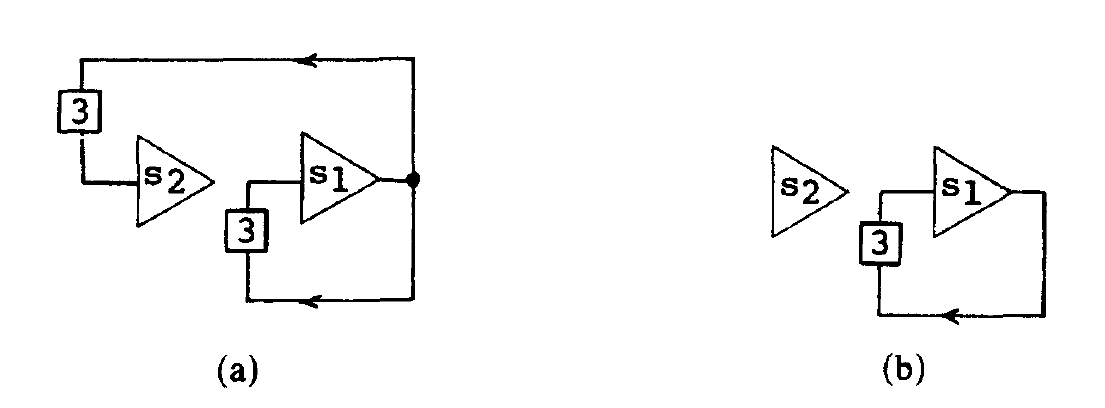
\includegraphics[width=0.7\linewidth]{pictures/fig3ab.png}
	\caption{Два эквивалентных КА: упрощение путём примарного разложения}
	\label{fig3ab}
\end{figure}

\section{Циклическое разложение}
В силу теоремы 4.5 мы можем предположить без потери общности, что начнём с локального артинова кольца $(R,M)$ и примарного $E \in \Mod_n(R[x])$. В общем случае разложение $E$ на циклические $R[x]$-модули не представляется возможным. Приведём следующий пример.

\paragraph{Пример 5.1}
Пусть $R = \mathbb{Z}_4, E = e_1 R \oplus e_2 R$. Два КА на рисунке \ref{fig4} эквивалентны. Они соответствуют матрицам ${ A =
	\begin{pmatrix}
		1 & 2\\
		2 & 3
\end{pmatrix}}, ~
{ A' =
	\begin{pmatrix}
		3 & 2\\
		2 & 1
\end{pmatrix}}
$.

Перебирая все преобразования $GL_2(\mathbb{Z}_4)$, мы можем убедиться в том, что $\{A, A'\}$ --- это \hl{класс подобия (similarity-class)} $A$. И ни $A$, ни $A'$ не являются \hl{представлениями (representations)} циклических модулей. \\

\begin{figure}[h]
	\centering
	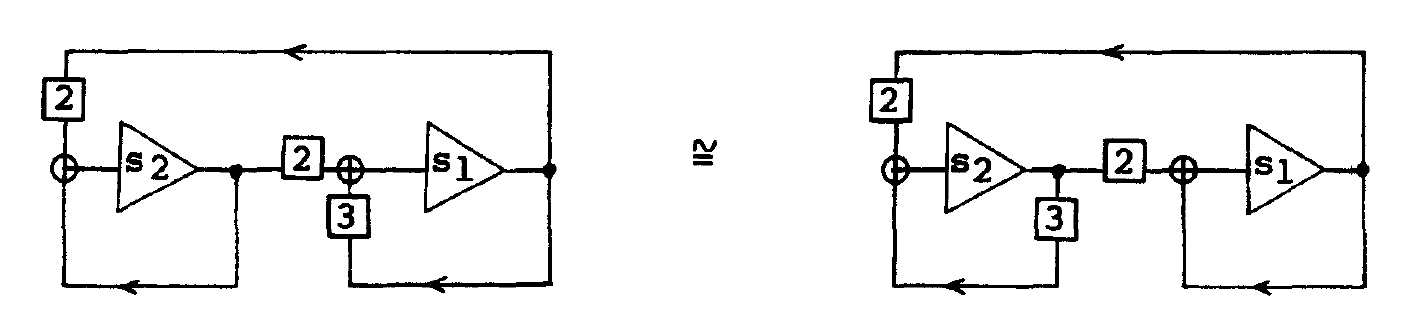
\includegraphics[width=0.7\linewidth]{pictures/fig4.png}
	\caption{Контрпример: КА над $\mathbb{Z}_4$, который неразложим на сдвиговые регистры}
	\label{fig4}
\end{figure}

Поэтому мы определяем более слабое условие, чем прямая сумма. Пусть $L_i$ --- это $R[x]$-подмодули $E$ $(i = 1,...,k)$ такие, что $\sum_{i=1}^{k} L_i = E$.

\paragraph{Определение 5.2}
Сумма $E = \sum_{i=1}^{k} L_i$ называется прямой суммой по модулю $M$, если $\overline{E} \cong \bigoplus_{i=1}^{k} \overline{L_i}$, и обозначается как $\dirsummod{M}_{i=1}^{k} L_i$.

Легко заметить, что $E = \dirsummod{M}_i L_i$, если $(L_i + M E) \cap \sum_{j \ne i} L_j ~ \subset ~ M E$. Напомним, что $R[x]$-модуль $E$ называется циклическим, если $E$ может быть порождён одним элементом; тогда мы имеем $E \cong R[x]/\Ann(E)$.

\paragraph{Лемма 5.3}
{\itshape
Для указанных выше $(R, M)$ и $E$ существуют нормированные и неприводимые $\alpha_i \in \overline{R}[x]$ и $s_i \in \mathbb{N} (i = 1,...,k)$ такие, что $\overline{E} \cong \bigoplus_{i=1}^{k} L'_i$ и $L'_i \cong \overline{R}[x]/(\alpha_i^{s_j})$.
}

\paragraph{Доказательство}

Поскольку $e$ является $R[x]$-модулем, мы можем применить структурную теорему для конечнопорождённых модулей над \hl{областью главных идеалов(principial ideal domain)} $\overline{R[x]} = R[x]/M[x] = (R/M)[x]$ (пример в работе \cite{bib3}). Из того, что $e$ примарный, получается что $\overline{E}$ и, следовательно, все подмодули $L'_i$ тоже примарны. Примарный идеал в $\overline{R[x]}$ --- это мощность простого идеала $(\bar{\alpha}_i)^{s_i}$. $\Box$ \\


Эти $\bar{R}[x]$-подмодули $L'_i \subset \bar{E}$ могут быть \hl{подняты до (can be lifted to)} $R[x]$-подмодулей $L_i$ следующим образом. Пусть $e'_i \in L'_i$ порождает $L'_i$, а выбор $e_i \in \pi ^{-1} (e'_i) \subset E $ произволен: тогда $L_i := R[x] \cdot e_i (i = 1, ..., k)$. Каждый $L_i$ циклический по определению, но в общем случае не $R$-свободный. Поскольку $\pi ((L_i + M E) \cap \sum_{j \ne i}L_j) = L'_i \cap \sum_{j \ne i} L_j = 0$ мы доказали следующую теорему.

\paragraph{Теорема 5.4}
{\itshape
Пусть $(R, M)$ --- артиново локальное кольцо, и $E \in \Mod_n(R[x])$ --- примарный модуль. Тогда существуют циклические $R[x]$-модули $L_i \subset E (i = 1, ..., k)$ такие, что $E = \dirsummod{M}_{i = 1}^k L_i$ (сумма по модулю $M$).
}


\paragraph{Теорема 5.5}
{\itshape
Для $(R, M)$ и $E$ указанных выше:
$$
\begin{aligned}
E \cong \oplus_{i = 1}^{k} L_i &  \Leftrightarrow L_i ~~ \text{является R-свободным} ~~ (i = 1, ..., k) \\
&  \Leftrightarrow   \Ann_{R[x]}(L_i) ~~ \text{является главным идеалом} ~~ (i = 1, ..., k).
\end{aligned}
$$
}

\paragraph{Доказательство}
(а) ($\Rightarrow$): $E$ --- $R$-свободный модуль, а $L_i$  --- прямое слагаемое $E$, следовательно, $L_i$ является \hl{$R$-проективным (R-projective)}, и тогда можно использовать теорему 3.8.

($\Leftarrow$): Из теоремы 3.8 мы можем заключить, что $L_1 \cap \sum_{i>1} L_i$ является $R$-свободным, а из определения суммы по модулю $M$, мы знаем, что
$$
(L_1 + M E) \cap \sum_{i>1} L_i ~~ \subset ~~ ME ~~~~ \Rightarrow ~~~~ L_1 \cap \sum_{i>1} L_i = 0.
$$

Теперь продолжим для $\sum_{i>1} L_i$ по индукции.

(б) Пусть $i = 1, ..., k$ произвольно, $e$ порождающий в $L_i$ и $d:=d_i$, тогда $B:={e, xe, ..., x^{d-1}e}$ --- $R$-базис в $L_i$.

($\Rightarrow$): $x^d e = \sum_{j = 0}^{d - 1} a_j (x^j e) \in L$ \hl{подразумевает (в оригинале implying --- причастие)}, что $\alpha := x^d - \sum_{j=0}^{d-1} a_j x^j \in \Ann(L)$ и $\alpha$ имеет степень $d$. Согласно лемме 3.9, $\Ann(L) = (\alpha) + N$ при $N \subset M[x]$. Если $N \ne 0$, тогда $\exists 0 \ne \beta \in N, \deg(\beta) < d$ (лемма 3.9), но это приводит к противоречию с тем, что базис $B$ линейно независим.

($\Leftarrow$): Без потери общности, $\Ann(L_i)$ порождён элементом $\alpha \in R[x]$ с ненулевым старшим коэффициентом. Очевидно, что $\deg(\alpha) = d$. Поскольку $\Ann(L_i)$ не содержит многочленов меньшей степени, в $B$ не существует зависимостей между элементами, следовательно, $B$ является базисом. $\Box$


\paragraph{Пример 5.6}
Пусть $R = \mathbb{Z}_4, ~ E=\bigoplus_{i=1}^4 e_i \cdot \mathbb{Z}_4$. Автомат на рисунке \ref{fig5abc} соответствует матрице переходов $${ A =
	\begin{pmatrix}
		0 & 1 & 0 & 2\\
		1 & 2 & 2 & 0\\
		0 & 0 & 0 & 1\\
		4 & 0 & 1 & 0
\end{pmatrix}}.$$ $\Ann(E) = ((x^2 - 1)(x^2 - 2x - 1), 4(x^2 - 1))$.

Следуя выводу и нотации теоремы 5.4, мы получаем $\bar{R}[x] = \mathbb{Z}_2 [x]$, $\bar{E} = \bigoplus_{i=1}^4 \bar{e}_i \mathbb{Z}_2$ и $\Ann_{\mathbb{Z}_2[x]}(\bar{E}) = (x^2 + 1)$. $L'_1 = L_{\mathbb{Z}_2}(\bar{e}_1, \bar{e}_2)$, аналогично, $L'_2 = L_{\mathbb{Z}_2}(\bar{e}_3, \bar{e}_4)$. Теперь выберем $\hatei{1} := e_1 + 2e_3, \hatei{2} := 3e_3$ и найдём, что оба
$$ L_1 = L_{\mathbb{Z}_8[x]}(\hatei{1}) =  L_{\mathbb{Z}_8}(\hatei{1}, x \hatei{1}, (4x + 4) \hatei{2}), $$
$$ L_2 = L_{\mathbb{Z}_8}(\hatei{2}, x \hatei{2}, (4x + 4) \hatei{1})$$
не являются $\mathbb{Z}_8$-свободными.

\begin{figure}[h]
	\centering
	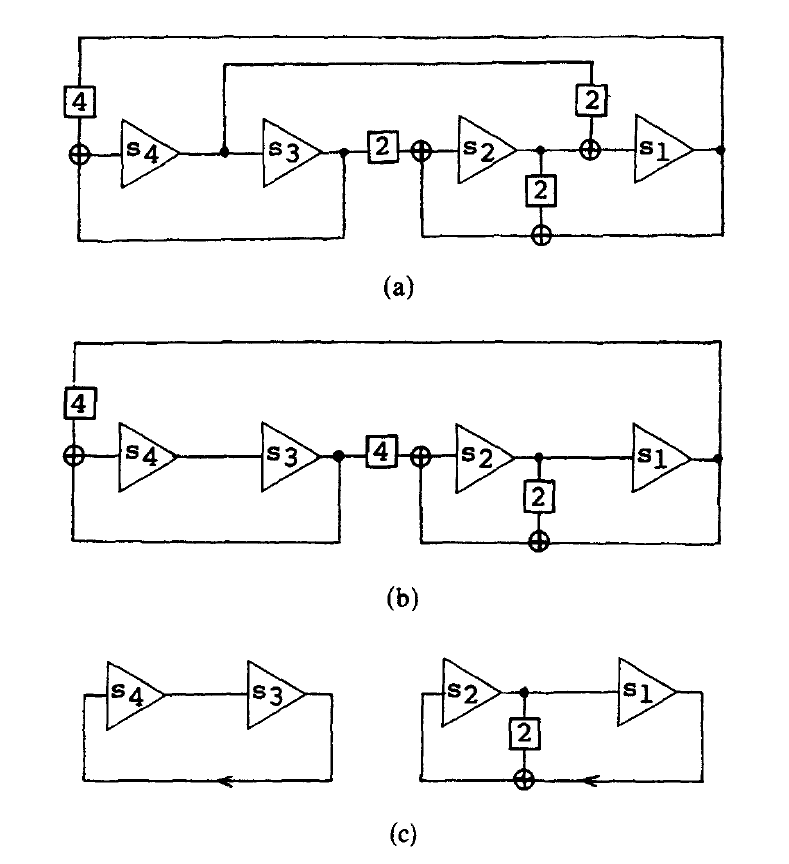
\includegraphics[width=0.7\linewidth]{pictures/fig5abc.png}
	\caption{Три эквивалентных КА: упрощение с помощью циклического разложения}
	\label{fig5abc}
\end{figure}

Относительно нового базиса $\{\hatei{i}\}$ мы получаем новую матрицу переходов $A^*$
$$
\begin{array}{cc}
	A^* = \begin{pmatrix}
		0 & 1 & 0 & 0 \\
		1 & 2 & 4 & 0 \\
		0 & 0 & 0 & 1 \\
		4 & 0 & 1 & 0
	\end{pmatrix} = \begin{pmatrix}
	0 & 1 & 0 & 0 \\
	1 & 2 & 0 & 0 \\
	0 & 0 & 0 & 1 \\
	0 & 0 & 1 & 0
	\end{pmatrix}
	+ &
	\begin{pmatrix}
		0 & 0 & 0 & 0 \\
		0 & 0 & 4 & 0 \\
		0 & 0 & 0 & 0 \\
		4 & 0 & 0 & 0
	\end{pmatrix}. \\
	~ & \text{\scriptsize "<твист-матрица">}
\end{array}
$$

Поскольку $L_1$ и $L_2$ не являются $\mathbb{Z}_8$-свободными, два сдвиговых регистра соединены, но со следующими ограничениями:

\begin{enumerate}
	\item[(1)] они соединены только элементами нильрадикала (составляющими "<твист-матрицы">);
	\item[(2)] они заканчиваются только в первых элементах задержки (с наивысшим индексом) каждого сдвигового регистра.
\end{enumerate}

\paragraph{Определение 5.7}
Примарный $R$-свободный $R[x]$-модуль называется скрученным, если он не изоморфен прямой сумме циклических $R[x]$-модулей. \\

Теорема 5.4 даёт нам необходимые и достаточные условия для определения скручен ли модуль или нет. Но у нас существует неприятная ситуация, в которой подмодули $L_i$ зависят от выбора $e_i \in \pi^{-1}(e'_i)$. Для одних $e_i$ $L_i$ будут циклическими, а для других нет. В приведённом ниже следствии мы следуем "<алгоритмическому"> подходу к проблеме отсутствующей независимости.


\paragraph{Следствие 5.8}
{\itshape
	Для $(R, M)$ и $E$ указанных выше, $E = \dirsummod{M}_{i=1}^m L_i$, пусть $\alpha_i \in R[x]$ --- нормированный многочлен, для которого $(\overline{\alpha_i}) = \Ann(L'_i) \subset \bar{R}[x]$. Тогда $E$ не является скрученным, если существуют $\nu_i \in M[x] (i = 1, ..., k)$ такие, что $(\alpha_i + \nu_i)L_i \subset (\alpha_i + \nu_i) M E$. Если $E$ не скрученный, тогда $\Ann(E) = \bigcap_{i=1}^k (\alpha_i + \nu_i)$. 
}

\paragraph{Доказательство}
($\Rightarrow$): Очевидно по теореме 5.5: мы зададим $\nu_i := 0$.

($\Leftarrow$): Существует $m_i \in M E$ такой, что $(\alpha_i + \nu_i)e_i = (\alpha_i + \nu_i) m_i$ для $L_i$-порождающих $e_i$ подразумевает $(\alpha_i + \nu_i)(e_i - m_i) = 0$. Определим $L_i^0 := R[x](e_i - m_i)$; $L_i^0$ является $R$-свободным, и $\overline{L_i^0} = L'_i$ подразумевает $E = \sum_{i = 1}^{k} L_i^0$, а теорема 5.4 завершает доказательство:

$$
\Ann(E) = \Ann\left(\sum_i L_i \right) = \bigcap_i \Ann(L_i) = \bigcap_i (\alpha_i + \nu_i). ~~~~ \Box
$$

\paragraph{Пример 5.6} \textit{(Продолжение)}.
Зададим $\alpha_1 = x^2 + 1 \in \mathbb{Z}_8[x],~ \nu_1 = nx + m ~ (n, m \in (2) \subset \mathbb{Z}_8)$. $(x^2 + nx + m + 1)\hatei{1} = \hatei{1} ((m+2) + x(n+2)) + 4 \hatei{2}$, и для $n = m = 6$ мы получаем $(x^2 - 2x - 1)\hatei{1} = (x^2 - 2x - 1) 2x \hatei{2} = 4 \hatei{2}$. Следовательно, для нового выбора $\hatei{1}^0 := \hatei{1} - 2 x \hatei{2} = e_1 + 2 e_3 + 2 e_4$, $~L_1^0$ является $\mathbb{Z}_8$-свободным, $~\Ann(L_1^0) = (x^2 - 2x - 1)$. Аналогичным образом если мы выберем $\hatei{2}^0 := \hatei{2} - 2x \hatei{1} = e_3 + 2 e_2$, то $L_2^0$ тоже становится $\mathbb{Z}_8$-свободным, $~\Ann(L_2^0) = (x^2 - 1)$. Матрица переходов $A^*$ принимает вид $$ A^* = \begin{pmatrix}
	0 & 1 & 0 & 0 \\
	1 & 2 & 0 & 0 \\
	0 & 0 & 0 & 1 \\
	0 & 0 & 1 & 0
\end{pmatrix},$$ соответствуя конечному автомату на рисунке \ref{fig5abc}(c).
$$
\begin{aligned}
E \text{ не скручен } ~~ \Rightarrow ~~ \Ann(E) & = (x^2 - 2x -1) \cap (x^2 - 1) \\
& = ((x^2 - 2x -1)(x^2 - 1), 4(x^2 - 1)).
\end{aligned}
$$

\section{Специальный случай с рекурсивным критерием}

Мы продолжим рассматривать проблему предыдущего раздела, где $(R, M)$ --- это локальное артиново кольцо, а $E \in \Mod_n (R[x])$ --- примарный модуль. Для формулировки специального случая, нам необходимо сначала дать определение. Напомним, что согласно теореме 5.4 $E = \dirsummod{M}_{i=1}^k L_i$, где циклические $R[x]$-модули $L_i \subset E (i = 1, ..., k)$.


\paragraph{Определение 6.1}
Примарный модуль $E = \dirsummod{M}_{i=1}^k L_i \in \Mod_n (R[x])$ называется \hl{полным степени $d$ (full of degree)}, если все $L_i$ имеют $d$ линейно независимых порождающих. \\

Другими словами, $\dim_{\bar{R}} (\overline{L_i}) = d ~~ (i = 1, ..., k)$. Конечный автомат, соответствующий \hl{полному модулю степени $d$ (full module of degree)} $d$, характеризуется постоянным числом $d$ элементов задержки в каждом сдвиговом регистре.

Пусть $A := R[x] / \Ann(E)$. Конечно, $E$ --- это $A$-модуль.

Эта часть имеет следующую мотивацию. Конечный автомат, соответствующий \hl{полному модулю (full module)}, состоит из сдвиговых регистров $\mathcal{A}_i ~ (i = 1, ..., k)$, а соединения между ними описываются "<твист-матрицей">. Мы хотим рассматривать сдвиговый регистр как "<векторный элемент задержки">, как элемент задержки $\mathcal{J}_i$ над $A$, а мультипликаторы в соединениях между  $\mathcal{J}_i$ как элементы $A$ (см. рисунок \ref{fig6ab}).

\begin{figure}[h]
	\centering
	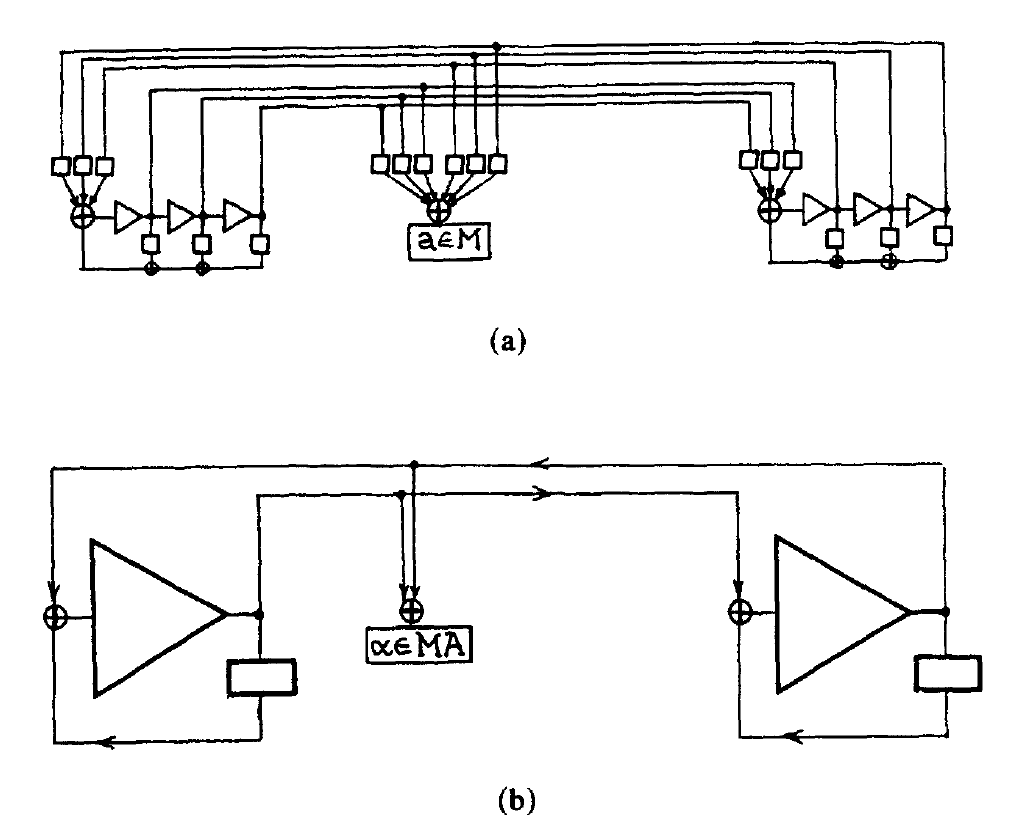
\includegraphics[width=0.7\linewidth]{pictures/fig6ab.png}
	\caption{(a) Диаграмма КА над $(R, M)$, соответствующего \hl{полному модулю степени (full module of degree)} 3. (b) Диаграмма эквивалентного КА над $A = R[x] / \Ann (E)$.}
	\label{fig6ab}
\end{figure}

Выберем \hl{минимальный набор (minimal set)} $A$-порождающих $\{e_1, ..., e_k\}$ из $E$. Поскольку каждый модуль является образом свободного модуля, мы имеем отображение $\rho : F \rightarrow E$ для свободного $A$-модуля $F$ с базисом $\{b_1, ..., b_k\}, ~ \rho(b_i) = e_i (i = 1, ..., k)$. Мы получаем короткую, чёткую последовательность
$$
0 \rightarrow \ker (\rho) \rightarrow F \overset{\rho}{\rightarrow} E \rightarrow 0.
$$

\paragraph{Лемма 6.2}
{\itshape
Пусть $E = \dirsummod{M}_{i=1}^k L_i$ \hl{полный $A$-модуль степени (full A-module of degree)} $d$. Тогда существует нормированный $\alpha \in A$ степени $d$ такой, что $\im (\alpha) \subset M E$. $\alpha$ уникален с точностью до многочленов степени $d - 1$ из $M A$.
}

\paragraph{Доказательство}
Для полного модуля мы всегда можем выбрать нормированный $\alpha \in A$, для которого $(\bar{\alpha}) = \Ann (\overline{L_i}) ~ (i = 1,...,k)$. $deg(\alpha) = deg(\bar{\alpha}) = dim_{\overline{R}}(\overline{L_i}) = d$. Для всех $e \in E, \pi(\alpha e) = \bar{\alpha} \bar{e} = 0$, следовательно, $e \in M E. ~~~ \Box$

Порождающие $\ker(\rho)$ определяются с помощью \hl{отношений (relations)} в $E$. Они имеют вид $a b_i = \sum_{j = 1}^{k} \beta_{ij} b_j ~ (i = 1, ..., k), ~ \alpha \in A$ нормирован, $\beta_{ij} \in M A$. Мы выбираем $\alpha$ в соответствии с леммой 6.2. Затем мы определим $h \in \Endom(F)$ как $h(b_i) := a b_i - \sum_{j=1}^{k} \beta_{ij} b_j ~ (i = 1, ..., k)$ и, таким образом, найдём точную последовательность
$$
F \overset{h}{\rightarrow} F \overset{\rho}{\rightarrow} E \rightarrow 0.
$$

Заметим, что $E \cong \coker(h)$. Теперь определим $f_\alpha := \alpha - h$.


\paragraph{Теорема 6.3}
{\itshape Пусть $E \in \Mod_n(A)$ полный степени $d$. Тогда следующие свойства эквивалентны:
	\begin{enumerate}
		\item $E$ не является скрученным с циклическими подмодулями ранга $d$ ($i = 1, ..., k$);
		\item $h$ \hl{диагонализируемый (diagonalisable)} с нормированными \hl{eigenvalue-polynomials of degree d (i = 1, ... k)}; % Прямо-таки Mindestlohndokumentationspflichtenverordnung из https://www.recht.bund.de/bgbl/1/2023/372/VO;
		\item $f_{\alpha} \in \Hom(F, MF)$ \hl{диагонализируемый (diagonalisable)}\hl{with eigenvalue-polynomials in MA of de-
		gree < d ( i = 1 , . . . , k ).}
	\end{enumerate}

}


\paragraph{Доказательство}
(1) $\Rightarrow$ (2): В лемме 3.9 и в доказательстве теоремы 5.5 мы использовали факт того, что $x^d \cdot \hatei{i} = \beta_i e_i, ~ \deg(\beta_i) < d \Rightarrow h(b_i) = (x^d - \beta_i) b_i)$, следовательно, $h$ является диагональным по отношению к базису $\{b_i\}$ и $\deg(x^d - \beta_i) = d$.

\hl{(2) $\Leftarrow$ (1)}: Пусть $h$ \hl{диагонализируемый (diagonalisable)}. Тогда существует преобразование базиса $t \in \Aut(F)$ такое, что $t^{-1} \cdot h \cdot t$ является диагональным.

$$
\begin{CD}
	 F 	@>h>> 			F 		@>\rho>>	E	@>>> 0\\
	 @VVtV 				@VVtV			@VV\hat{t}V	\\
	 F 	@>tht^{-1}>>	F		@>\rho>>	E	@>>> 0
\end{CD}
$$

В общем случае невозможно \hl{расширить $t$ на $E$ (extend t to E)} как $A$-гомоморфизм, потому что $t(\ker(\rho)) \not \subset \ker(\rho)$. Но достаточно рассматривать как (свободный) $R$-модуль. Тогда существует $\hat{t} \in \Aut_R (E)$, где $\rho t = \hat{t} \rho$. Начиная с $h(b_i) = \alpha b_i - \sum_j \beta_{ij} \cdot b_j$, мы получаем $(tht^{-1})(tb_i) = \alpha (tb_i) - \sum_j \beta_{ij} \cdot (tb_j) = \gamma_i \cdot (tb_i)$, поскольку $h$ \hl{диагонализируемый (diagonalisable)}. $\deg(\gamma_i) < d$. С учётом $\hatei{i}^0 : = \rho (t b_i)$, мы получаем $\gamma_i (e_i^0) = \gamma_i \rho (t b_i) = \rho \gamma_i (t b_i) = \rho (tht^{-1}) (t b_i) = \hat{t} (\rho h) t^-1 (t b_i) = 0$, так как $\rho h = 0$.

(2)$\Leftrightarrow$(3): Этот факт непосредственно следует из эквивалентности (1) и (2) и из определения $f_\alpha$. $\Box$

\paragraph{Нотация}
$E' := F/M^{z-1}F, R' := R[x]/ (Ann(E) + M^{z-1})$.

\paragraph{Теорема 6.4}
Пусть $(R, M)$ --- локальное артиново кольцо главных идеалов, $M = (m)$, $z$ --- \hl{нильпотентность (nilpotency)} $M$ и $E \in \Mod_n (R[x])$. Тогда существуют изоморфизмы
\begin{itemize}
	\item[(а)] $\phi: \Hom_R(F, MF) \rightarrow \Endom_{R'}(E')$;
	\item[(б)] $\psi: \Aut_R (F)/(1+\Hom(F, M^{z-1}F)) \rightarrow \Aut_{R'}(R')$;
	\item[(в)] $\phi$ и $\psi$ \hl{коммутируют (commute)} с действием группы автоморфизмов на кольце эндоморфизмов, особенно, $$\bar{\phi} : \Hom_R(E, ME)/ \Aut_R(E) \cong \Endom_{R'}(E') / \Aut_{R'}(E').$$
\end{itemize}
 
 
\paragraph{Доказательство}
Для данного доказательства пусть $H:= \Hom(F, M^{z-1} F)$

(a) Пусть $m : = F \rightarrow (m)E$ (умножение на $m$). Тогда $\ker (m) = M^{z-1}$ и $\bar{m} : E' \cong (m)E$. Аналогично мы можем связать $f : E\rightarrow(m)E$ с $\bar{f} : E' \rightarrow (m)E$ и, таким образом, определить $f' := \phi(f) := \bar{m}^{-1} \cdot \bar{f} \in \Endom(E')$, где $f'\pi = \pi f$.

$\phi$ --- мономорфизм, потому что $\ker(\phi) = \{f \in \Hom(E, ME) | \bar{f} = 0\} = 0$.

$\phi$ --- эпиморфизм: Пусть $f' \in \Endom(E')$ будет произвольным:
$$
\begin{tikzcd}
	E	\ar{d}[']{\pi} \arrow{r}{mf}	& (m)E \\
	E' 	\rar{f'}							& E' \ar{u}{\cong}[']{\bar{m}}
\end{tikzcd}
$$

Поскольку $E$ является свободным, $f'$ может быть \hl{поднят по $\pi$ (be lifted along $\pi$)} для получения $mf \in \Endom(E)$. $\phi^{-1}(f') := mf$ подразумевает $\phi(mf) = \bar{m}^{-1} \cdot (mf) = \pi \bar{f} = f'$.

(б) Определим $\psi' : \Aut(E) \rightarrow \Aut(E')$ с помощью $\psi (g) := g'$, где $\pi g = g' \pi$ для $g \in \Aut(E)$. $\psi'$ корректно определено и является эпиморфизмом (как в асти (а)). \hl{Прим.: в начале абзаца вероятно опечатка во второй формуле.} 

$$
\begin{tikzcd}
	E	\ar{d}[']{\pi} \arrow{r}{g}	& E \ar{d}{\pi} \\
	E' 	\rar{g'}			& E'
\end{tikzcd}
$$

$\psi' (g) = 1_E  \Leftrightarrow \pi = \pi g \Leftrightarrow 1_E - g \in \ker(\pi) \Leftrightarrow 1_E - g \in H$. Следовательно, $\ker(\psi') = 1 + H$ и $\psi$ является мономорфизмом.


$$
\begin{tikzcd}
	\Aut(E) \ar{d} \ar{rd}{\alpha} & \\
	\Aut(E) / (1+H) \rar{\alpha} \dar{\cong}[']{\psi}& \Endom(\Hom(E,ME)) \dar{\cong}[']{\phi^*} \\
	\Aut(E') \rar{\alpha}&  \Endom(\Endom(E'))
\end{tikzcd}
$$

(в) $\alpha$ --- это действие $g \in \Aut(E)$ на $f \in \Endom(E), ~ \alpha (g) f : = g^{-1} f g \in \Endom(E)$. Пусть $\bar{g} \in \Aut(E)/(1+H)$ и $mf \in \Hom(E, ME)$. Тогда $\phi^* \alpha (\bar{g})(mf) = \phi^*(\bar{g}^{-1}mf\bar{g}) = (\bar{g}^{-1} f \bar{g})'$ и $\alpha \psi (\bar{g})(f') = (\bar{g}')^{-1} f' \bar{g}'$. Из-за линейности $f, g$ и $\pi$ получаем $(\bar{g}^{-1} f \bar{g})' = (\bar{g}')^{-1}f'\bar{g}'$. $\Box$


\paragraph{Теорема 6.5}
{\itshape
Пусть $(R,M )$ --- артиново локальное кольцо главных идеалов, а $E \in \Mod_n(R[x])$ \hl{является полным степени $d$ (full of degree d)}. $E$ не скручен тогда и только тогда, когда $f' := \phi (f) \in \Endom_{R'}(E')$ \hl{диагонализируемый (diagonalisable)}.
}

\paragraph{Доказательство}
Согласно теореме 6.3, нам необходимо показать, что $\phi: \Hom(F,MF) \rightarrow \Endom(E')$ "<сохраняет диагональность">. Пусть $B:=\{b_1, ..., b_k\}$ --- базис в $F$, $\pi : F \rightarrow E' = F/M^{z-1}F$ --- \hl{канониеское отображение (canonical projection)} и $\pi(B)$ --- базис в $E'$.

$$
\begin{tikzcd}
	A \dar[']{\pi} & F \dar[']{\pi} \rar{f_\alpha} & MF \\
	R' & E' \rar{f'} & E' \uar{\cong}[']{m}
\end{tikzcd}
$$

Теорема непосредственно следует из того факта, то $\pi$ и $m$ являются диагональными по отношению к $B$. $\Box$



\paragraph{Пример 6.6}
Пусть $R = \mathbb{Z}_9, E= \bigoplus_{i=1}^6 e_i \cdot \mathbb{Z}_9$. Мы хотим применить теоремы данного раздела к КА, который представлен на рисунке \ref{fig7abcd}(a). Матрица переходов задаётся относительно базиса $\{e_1, ..., e_6\}$ следующим образом:

$$
f = \begin{pmatrix}
	 0& 1& 0& 0& 0& 0\\
	 5& 6& 0& 0& 3& 3\\
	 0& 0& 0& 1& 0& 0\\
	 3& 6& 2& 0& 6& 3\\
	 0& 0& 0& 0& 0& 1\\
	 0& 0& 0& 0& 8& 0\\
\end{pmatrix}.
$$

\begin{figure}[h]
	\centering
	\includegraphics[width=0.75\linewidth]{pictures/fig7abcd.png}
	\caption{(a) КА над $\mathbb{Z}_9$. (b) Соответствующий КА над $\mathbb{Z}_3[x]/\Ann(E)$. (c) Разложение над $\mathbb{Z}_3[x]/\Ann(E)$. (d) Разложение на сдвиговые регистры над $\mathbb{Z}$.}
	\label{fig7abcd}
\end{figure}

$\Ann(E) = ((x^2+1)^2,3(x^2+2))$. Выберем $\alpha = x^2 - 2$. Над $R' = \mathbb{Z}_3 [x] / (x^2 + 1)$ мы имеем КА на рисунке \ref{fig7abcd}(b) с матрицей переходов $$
f' = \begin{pmatrix}
	1+2x&	0&	1+x\\
	1+2x&	0&	2+x\\
	0&		0&	2\\
\end{pmatrix}.
$$

$f' \in \Endom(E')$ предполагает определение $R'[y]$-модульной структуры на $E'$ с помощью $y \cdot e := f' \cdot e (\forall e \in E')$. Примарное разложение $E' \in \Mod_3(R'[y])$ показывает, что $f'$ является \hl{диагонализируемым (diagonalisable)} с помощью $t\in \Aut(E')$; мы получаем $f'^*$ и КА на рисунке \ref{fig7abcd}(c).

$$
f^* = \begin{pmatrix}
	1+2x&0&0\\
	0&0&0\\
	0&0&2\\
\end{pmatrix}
$$

Действие $\psi^{-1}(t)$ на $f$ даёт $f^*$, соответствующую КА, который изображен на рисунке \ref{fig7abcd} и является параллельным соединением сдвиговых регистров.

$$
f^* = \begin{pmatrix}
	0&1&0&0&0&0\\
	5&6&0&0&0&0\\
	0&0&0&1&0&0\\
	0&0&2&0&0&0\\
	0&0&0&0&0&1\\
	0&0&0&0&8&0\\
\end{pmatrix}.
$$

$E$ не скручен, следовательно,
$$
E \cong \mathbb{Z}_9[x] / (x^2 + 3x + 4) \oplus \mathbb{Z}_9[x]/(x^2-2) \oplus \mathbb{Z}_9[x] / (x^2 + 1).
$$

\paragraph{Лемма 6.7}
{\itshape
Пусть $(R, M)$ --- локальное артиново кольцо, и $E \in \Mod_n (R[x])$ примарный. Тогда $R'$ является локальным артиновым кольцом, а $\Rad(R) = \Rad(\Ann(E))/(\Ann(E) + M^{z-1})$.
}

\paragraph{Доказательство}
Поскольку каждый \hl{простой (prime)} идеал содержит нильрадикал, достаточно показать, что $\Rad(R')$ является \hl{максимальным (maximal)} идеалом.

$$ \begin{aligned}
\Rad(R') &= (\Rad(R[x]) + \Rad(\Ann(E)+M^{z-1}))/(\Ann(E)+M^{z-1}) \\
		&= \Rad(\Ann(E)) / (\Ann(E)+M^{z-1}).
\end{aligned}$$

Таким образом,
$$
R' / \Rad(R') = R[x] / \Rad(\Ann(E)+M^{z-1}) \cong R[x] / (M[x] + (\alpha)),
$$
согласно лемме 3.9, где $\alpha$ --- нормированный и фундаментально несократимый многочлен. Следовательно, $R'/\Rad(R') = \overline{R}[x]/(\bar{\alpha})$, которое является полем. $\Box$



\pagebreak
\begin{thebibliography}{99}
	
	\bibitem{bib1}
	M.F. Atiyah and I.G. MacDonald,
	Introduction to Commutative Algebra
	(Addison-Wesley, Reading, MA, 1969).
	
	\bibitem{bib2}
	W.S. Ching and B.F. Wyman,
	Duality and the regulation problem for linear systems over commutative rings,
	J. Comput. System Sci. 14 (1977) 360-368.

	\bibitem{bib3}	
	T. Hungefford,
	Algebra
	(Holt, Rinehart \& Winston, New York, 1974).
	
	\bibitem{bib4}	
	R.E. Kalman, P.L. Falb and M.A. Arbib,
	Topics in Mathematical System Theory
	(McGraw-Hill, New York, 1969).
	
	\bibitem{bib5}
	P. Khargonekar, On Matrix Fraction Representation for Linear Systems over Commutative Rings
	(Center of Math. System Theory, Univ. of Florida, 1980).
	
	\bibitem{bib6}	
	M. Magidin and A. Gill,
	Decomposition of linear sequential circuits over residue rings,
	J. Franklin Inst. 294 (1972) 167-180.
	
	\bibitem{bib7}	
	M. Magidin and A. Gill,
	Singular shift registers over residue class rings,
	Math. Systems Theory 9(4) (1976) 345-358.
	
	\bibitem{bib8}	
	G. Nandi and C. Nolte,
	Duality for systems over rings,
	Inform. Control 50. (1981) 128-132.
	
	\bibitem{bib9}	
	B. Reusch,
	Lineare Automaten
	(Bibliographisches Institut, Mannheim, 1969).
	
	\bibitem{bib10}	
	J.R. Silvester,
	Introduction to Algebraic K-theory
	(Chapman \& Hall, London, 1981).
	
	\bibitem{bib11}	
	E. Snapper,
	Completely primary rings,
	Ann. of Math. 52 (1950) 666-693.
	
	\bibitem{bib12}	
	E.D. Sontag,
	Linear systems over commutative rings, Ricerche Automat.
	7(1) (1976) 1-34.
	
	\bibitem{bib13}
	B.L. van der Waerden,
	Algebra 2
	(Springer, Berlin, 1967).
	
\end{thebibliography}


\end{document}